\question{{\it Aussagenlogische Gesetze}}

Beweisen Sie folgende aussagenlogische Gesetze mit Hilfe von Wahrheitstafeln:
\begin{enumerate}
\item $(a\wedge(b\wedge c))\Leftrightarrow((a\wedge b)\wedge c)$
\item $(a\vee(b\vee c))\Leftrightarrow((a\vee b)\vee c)$
\item $(a\Rightarrow b)\Leftrightarrow(\neg a\vee b)$
\item $(p\Rightarrow q)\Leftrightarrow(\neg q\Rightarrow\neg p)$
\item $(r\Leftrightarrow s)\Leftrightarrow((r\Rightarrow s)\wedge (s\Rightarrow r))$
\item $(a\wedge(b\vee c))\Leftrightarrow((a\wedge b)\vee(a\wedge c))$
\item $(a\vee(b\wedge c))\Leftrightarrow((a\vee b)\wedge(a\vee c))$
\item $((p\Rightarrow q)\wedge(q\Rightarrow r)\wedge(r\Rightarrow p))\Leftrightarrow((p\Leftrightarrow q)\wedge(q\Leftrightarrow r))$
\end{enumerate}



\question{{\it Aussagen mit Quantoren}}

Übersetzen Sie folgende Aussagen in umgangssprachliche Sätze bzw. umgekehrt, wobei $s(x)$ für ``$x$ ist ein Snark'', $b(x)$ für ``$x$ ist ein Boojum'', $f(x,y)$ für ``$x$ findet $y$'' stehen möge:
\begin{enumerate}
\item $\exists x~(s(x)\wedge b(x))$
\item $\exists x~\exists y~(s(y)\wedge f(x,y))$
\item $\forall x~b(x)\Rightarrow (s(x)\wedge \neg f(x,x))$
\item Jeder Snark, der von jemandem gefunden wird, ist ein Boojum.
\item Alle Boojums sind Snarks, aber nicht alle Snarks sind Boojums.
\item Jeder Boojum wird von jemandem gefunden.
\end{enumerate}



\question{{\it Einfache Operationen mit endlichen Mengen}}

Geben Sie für die folgenden Paare von Mengen $A$, $B$ jeweils $A\cup B$, $A\cap B$, $A\backslash B$, $B\backslash A$, $A\times B$ und $B\times A$ an:\\
\parbox{0.5\textwidth}{
\begin{enumerate}
\item $A=\{1,2,3\}$, $B=\{2,4,6,8,10\}$
\item $A=\{1,2,3,4\}$, $B=A$
\end{enumerate}}\parbox{0.5\textwidth}{
\begin{enumerate}\setcounter{enumi}{2}
\item $A=\{\emptyset,\{\emptyset\}\}$, $B=\{\emptyset,\{\emptyset,\{\emptyset\}\}\}$
\item $A=\{1,2,3,4\}$, $B=\{A\}$
\end{enumerate}}



\question{{\it Venn-Diagramme -- I}}

Zeichnen Sie jeweils ein Venn-Diagram, das die folgenden Verhältnisse zwischen Mengen widerspiegelt:
\begin{enumerate}
\item $B\subset A$, $C\cap A=\emptyset$
\item $A\cap B\not=\emptyset$, $\neg((A\subseteq B)\vee (B\subseteq A)$, $C\subset A$, $C\cap B=\emptyset$
\item $B\subset A$, $C\subset B$, $D\subset A$, $D\cap B=\emptyset$
\end{enumerate}



\question{{\it Venn-Diagramme -- II}}

\begin{center}
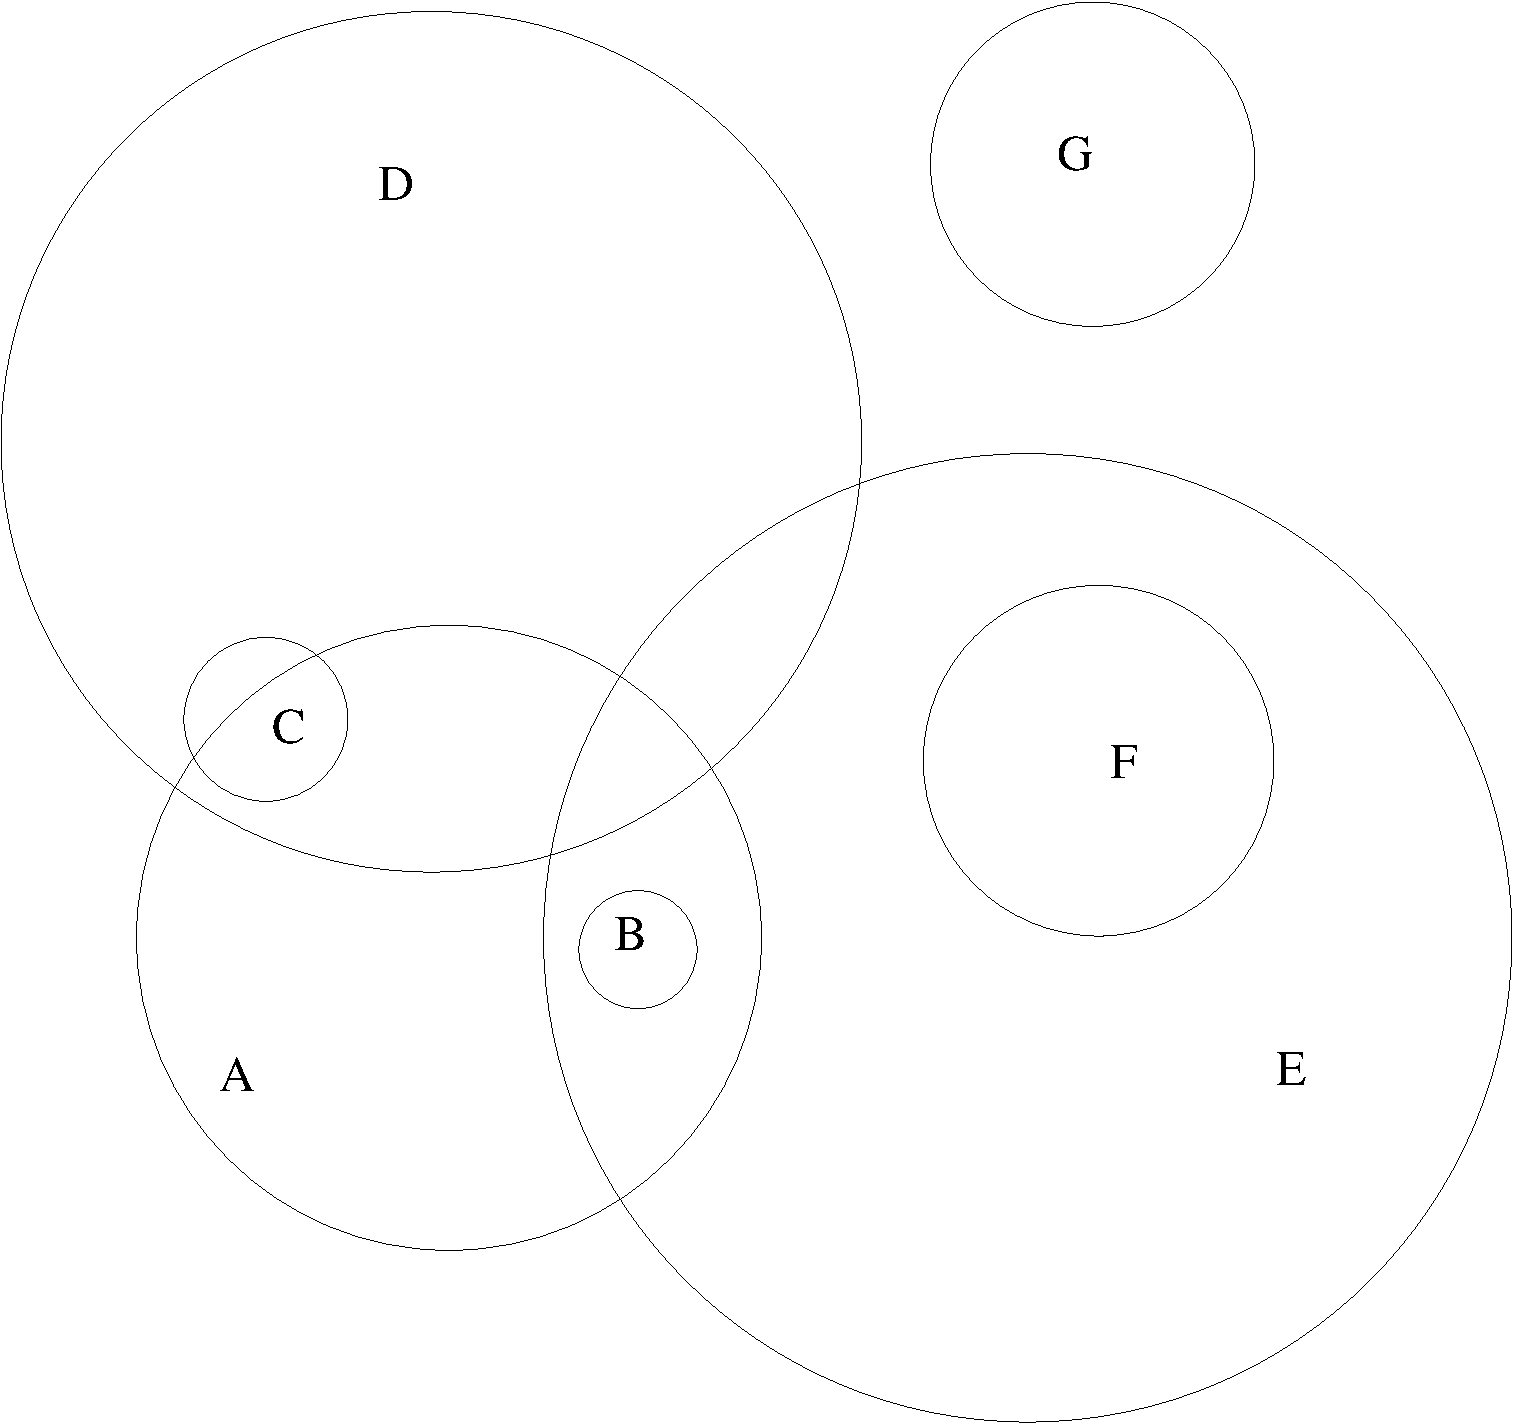
\includegraphics[width=0.65\linewidth,keepaspectratio=]{figures/vennproblemsheet.pdf}
\end{center}

Betrachten Sie das obenstehende Venn-Diagramm, und bestimmen Sie jeweils den Wahrheitswert der folgenden Aussagen:\\
\parbox{0.5\textwidth}{
\begin{enumerate}
\item $A\subseteq B$
\item $B\subset A$
\item $B\cap C=\emptyset$
\item $B\subseteq E$
\item $B\subset(A\cap E)$
\item $C\subseteq(A\cap D)$
\item $C\subseteq(A\cup D)$
\item $F\subset(E\backslash D)$
\end{enumerate}}\parbox{0.5\textwidth}{
\begin{enumerate}\setcounter{enumi}{8}
\item $C\subseteq(D\backslash A)$
\item $C\cap(D\backslash A)=\emptyset$
\item $F\subset(E\cup G)$
\item $C\subset(D\backslash E)$
\item $(C\cap A)\subset D$
\item $G\cup F=\emptyset$
\item $F\backslash E=\emptyset$
\item $(B\cap C)\subseteq (D\cap G)$
\end{enumerate}}



\question{{\it Mengentheoretische Gesetze}}

Beweisen Sie folgende Mengentheoretische Gesetze jeweils mit Hilfe des Extensionalitätsprinzips sowie der aussagenlogischen Gesetze aus Aufgabe 1:
\begin{enumerate}
\item $(A\cap(B\cap C))=((A\cap B)\cap C)$
\item $(A\cup(B\cup C))=((A\cup B)\cup C)$
\item $(A\cap(B\cup C))=((A\cap B)\cup(A\cap C))$
\item $(A\cup(B\cap C))=((A\cup B)\cap(A\cup C))$
\end{enumerate}



\question{{\it Zum Nachdenken und Diskutieren}}

\begin{enumerate}
\item Machen Sie sich den Unterschied zwischen dem umgangssprachlichen Gebrauch von ``wenn \ldots dann \ldots'' und der Bedeutung des aussagenlogischen $p\Rightarrow q$ an Beispielen wie ``Wenn Du Deine Suppe aufißt, bekommst Du Dessert.'' klar.
\item Erklären Sie ihrem Banknachbarn Ihre Einsichten.
\item Wiederholen Sie die beiden vorangehenden Schritte für umgangssprachlichen ``oder'' und aussagenlogisches $\vee$. Welche Unklarheit in der Bedeutung hat das umgangssprachliche ``oder''?
\end{enumerate}
